\chapter{Drone simulado}\label{cap.simulado}
En este capítulo se explica lo que se ha desarrollado para conseguir un comportamiento sigue persona con un drone simulado con el objetivo de ser incluido en la plataforma \textit{Kibotics} para enseñanza de robótica.

\section{Diseño}
El caso de la versión simulada es igual a la real, se compone de 2 partes claras (figura \ref{fig:esquemaReal}), la primera es la detección neuronal y la segunda los controladores PID.
\begin{figure}[H]
  \begin{center}
    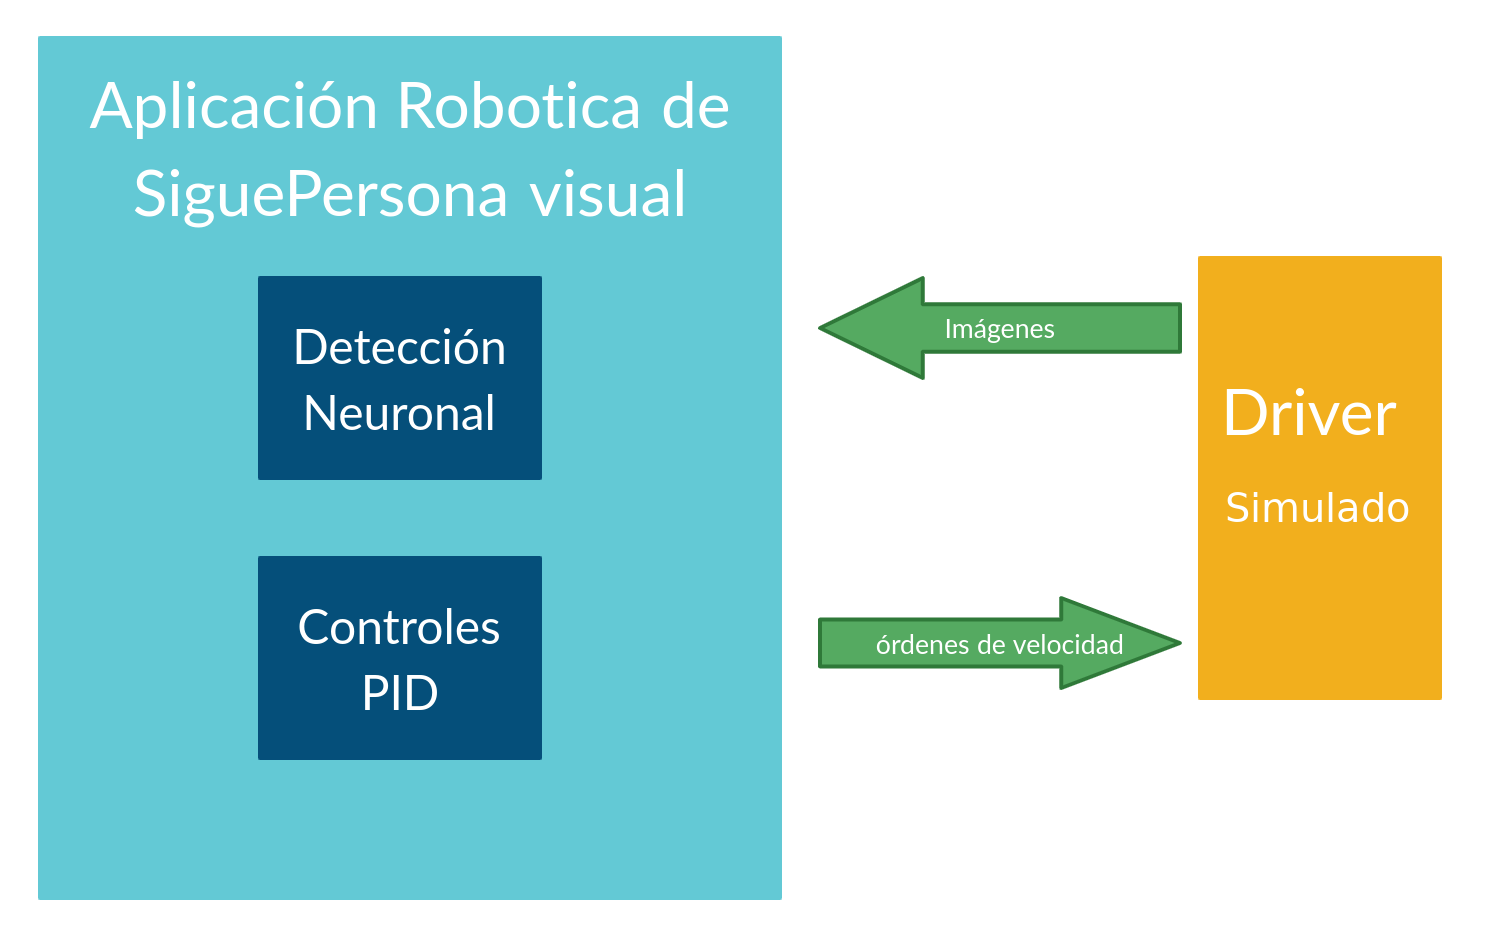
\includegraphics[width=0.7\textwidth]{figures/simulado/esquema.png}
		\caption{Diseño versión de simulador}
		\label{fig:esquemaSim}
		\end{center}
\end{figure}

La detección neuronal es un recubrimiento de la red neuronal que recibe las imágenes del driver y devuelve los \textit{bounding boxes}, puntuaciones y clases detectadas. 
La parte de los controladores usando los \textit{bounding boxes} calcula la velocidades y se las pasa al driver.
\section{Creación del escenario}
Lo primero es crear un escenario del simulador en el que haya un drone y una persona a la que seguir (figura \ref{fig:mundoSim}).
\begin{figure}[H]
  \begin{center}
    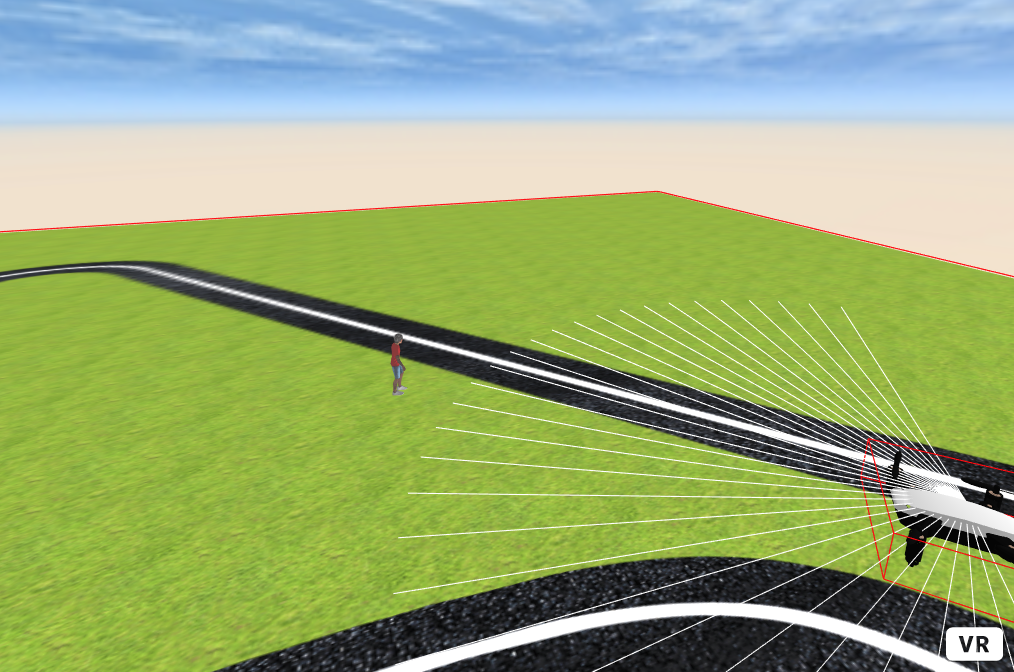
\includegraphics[width=0.7\textwidth]{figures/simulado/sim1.png}
		\caption{Mundo simulado}
		\label{fig:mundoSim}
		\end{center}
\end{figure}

Para ello se ha necesitado descargar varios modelos 3d de personas de la web mixamo \cite{mixamo} (figura \ref{fig:muneco}).
\begin{figure}[!htb]
\minipage{0.35\textwidth}
    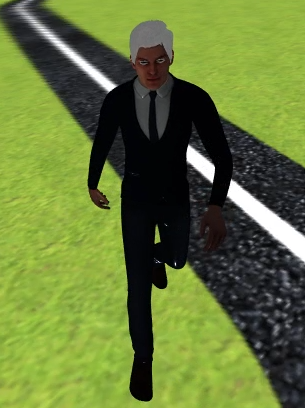
\includegraphics[width=\linewidth]{figures/simulado/muneco.png}
    \caption{Modelo 3D de persona}\label{fig:muneco}
\endminipage\hfill
\minipage{0.55\textwidth}
    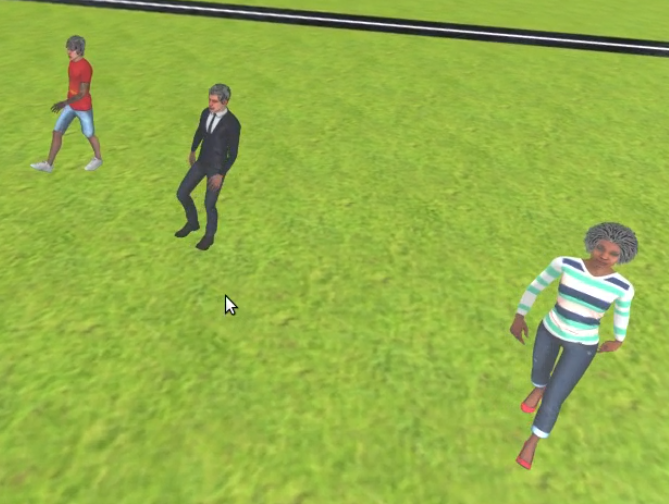
\includegraphics[width=\linewidth]{figures/simulado/persons.png}
    \caption{Modelos 3D seleccionados}\label{fig:persons}
\endminipage\hfill
\end{figure}

Los problemas que tenían estos modelos es que el simulador (\textit{websim}) los cargaba muy oscuros y con textura metálica, además de que ocupan mas de 100 MB. Para solucionar estos problemas se han cargado los modelos en \textit{Blender} para poder aclarar y quitar el metalizado de las texturas. Además se ha reducido el tamaño es estas para reducir el tamaño final de cada modelo a 3 MB.

Otro problema era que el modelo viene en un directorio con la forma de la persona en un fichero y las texturas separadas en varias imágenes. Así que se ha decidido guardarlo en un solo fichero \textit{\acrfull{glb}}. el resultado se puede ver en la figura \ref{fig:persons}.
\section{Comportamiento siguePersona visual}
EL comportamiento en el caso simulado es casi idéntico al real, cambiando cosas propias del lenguaje en cada caso.
\subsection*{Detección visual de la persona}
Debido a las limitaciones en la capacidad de procesamiento propias del interprete de \textit{Javascript} en este caso no se han probado con mas redes y se ha optado por la que mejores resultados ha dado en tiempos de ejecución de las pruebas reales, una \textit{SSD  Mobilenet  v2} (figura \ref{fig:mobilenet}).

Se trabaja con \textit{TensorflowJS  2.0.1}. Además se ha hecho un recubrimiento de la red para poderla usar más fácilmente permitiendo cargar la red siendo un grafo o un modelo de \textit{TensorflowJS}. También añade un postprocesado a la salida de la red.

Las red usada en \textit{Javascript} es básicamente las misma que en \textit{Python} pero con tres cambios importantes para mejorar rendimiento (figura \ref{fig:mobilenet2}):
\begin{itemize}
  \item Se elimina el postprocesado del modelo original.
  \item se suprime el \textit{NonMaxSuppression} multiclase original y se sustituye por uno de una sola clase
  \item las operaciones de \textit{NonMaxSuppression} se ejecutan en CPU para no perder tiempo en la carga de las texturas
\end{itemize}
\begin{figure}[H]
  \begin{center}
    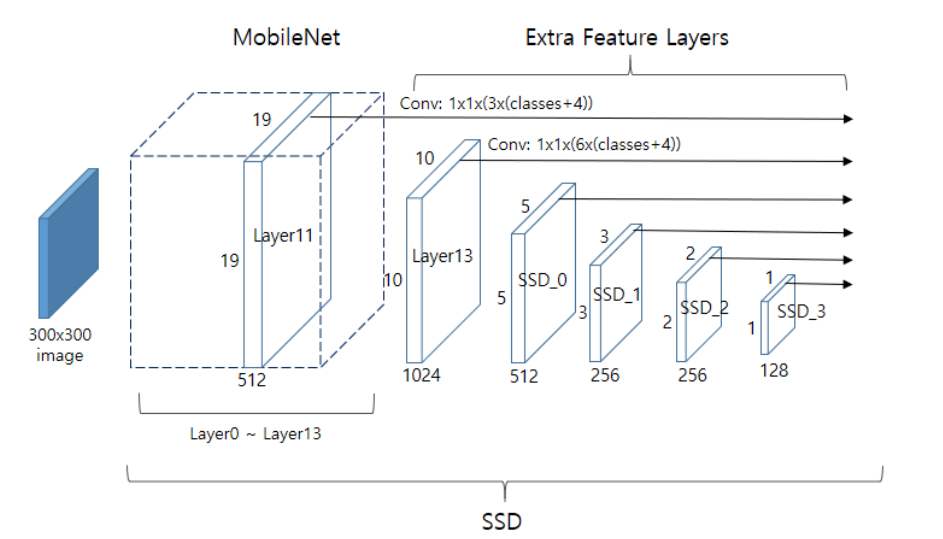
\includegraphics[width=0.6\textwidth]{figures/simulado/mobilenet.png}
		\caption{Esquema de una red Mobilenet ssd usada en \textit{TensorflowJS}}
		\label{fig:mobilenet2}
		\end{center}
\end{figure}

EL postprocesado en el caso de la versión simulada es la siguiente:
\begin{figure}[H]
  \begin{center}
    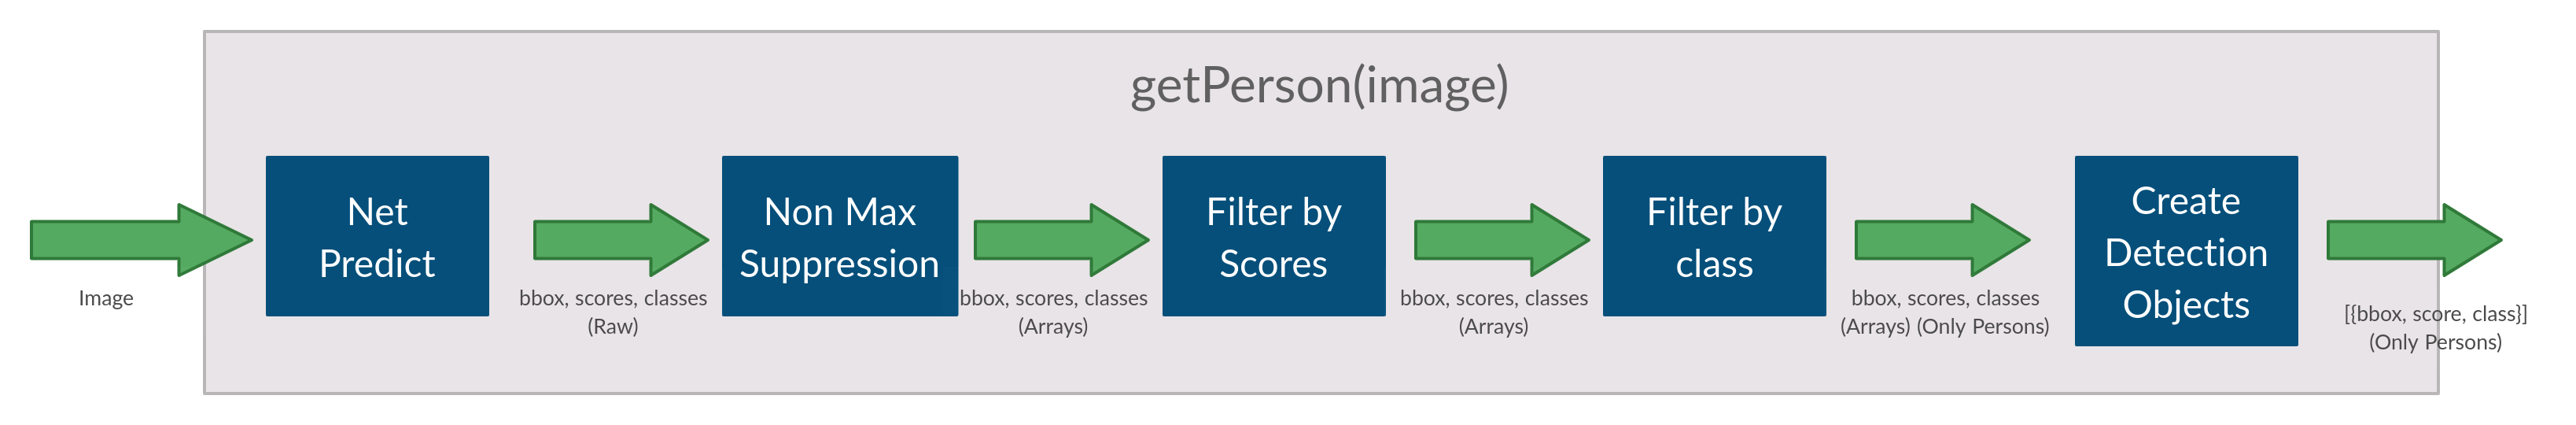
\includegraphics[width=1\textwidth]{figures/simulado/getPersonjs.png}
		\caption{función \textit{getPerson en JS}}
		\label{fig:getPersonjs}
		\end{center}
\end{figure}
\begin{itemize}
  \item Se pasa la salida de la red por una función \textit{NonMaxSuppression} monoclase para obtener ya las detecciones, puntuaciones y clases.
  \item Se filtran detecciones para eliminar las que tengan menos que el limite indicado por configuración.
  \item Se filtra por clase para quedarnos con las personas
  \item Se crea un \textit{array} de objetos que representan las detecciones (\textit{bounding box}, puntuación y clase)
\end{itemize}
Al final del postprocesado de la salida de la red se obtiene un \textit{array} con las detecciones representadas por un objeto que contiene\textbf{ \textit{bounding box}, puntuación y clase}.

Todo este procesamiento visual se ha incluido en el \textit{driver del drone simulado} para que pueda ser usado de manera sencilla desde las nuevas aplicaciones de robótica de los usuarios de \textit{Kibotics} con el simulador.
\subsection*{controles PID}
Una vez que se procesa la imagen recibida de el drone y se tienen las detecciones, se selecciona la persona con mayor puntuación y de su \textit{bounding box} se extrae posición central y el área. En este caso no se hace control vertical porque las imágenes recibidas no permiten un control aceptable en este eje.
\begin{figure}[H]
  \begin{center}
    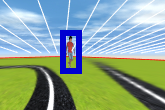
\includegraphics[width=0.7\textwidth]{figures/simulado/sim3.png}
		\caption{función \textit{Detección ideal}}
		\label{fig:sim3}
		\end{center}
\end{figure}

Para controlar el drone se va a hacer con dos velocidades, avance y giro horizontal. Para ello se utiliza un control PID (en este caso debido al funcionamiento del drone solo proporcional y derivativo) para cada una de las velocidades.
\subsubsection*{Control de avance}

En el caso de la velocidad de avance, se toma como referencia el área. Se fija un área objetivo para el \textit{bounding box}, si la obtenida es menor, se avanza y si es mayor se retrocede. Las constantes \textbf{proporcional y derivativa} en este caso son \textbf{0.01 y 0} respectivamente.

\subsubsection*{Control de giro horizontal o guiñada}

En este caso se toma como referencia la coordenada x del centro de la imagen. Si el \textit{bounding box} se mueve a la izquierda hay que girar a la izquierda y si se va a derecha igual. Las constantes \textbf{proporcional y derivativa} en este caso son \textbf{0.002 y 0.0001} respectivamente.

\section{Creación del \textit{dataset}}
En las primeras pruebas con el drone simulado se detecta que la detección del modelo es muy deficiente. No es capaz de detectarlo en más del 50\% de los fotogramas, lo que imposibilita un seguimiento aceptable. Por lo que se decide reentrenar la red de detección con un \textit{dataset} creado con capturas de imagen de cámara del drone\cite{github_dataset} (figuras \ref{fig:dataset1} y \ref{fig:dataset2}).
\begin{figure}[!htb]
\minipage{0.45\textwidth}
    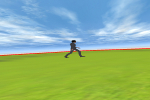
\includegraphics[width=\linewidth]{figures/simulado/person157.jpg}
    \caption{Ejemplo 1 del \textit{dataset}}\label{fig:dataset1}
\endminipage\hfill
\minipage{0.45\textwidth}
    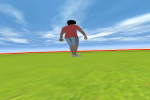
\includegraphics[width=\linewidth]{figures/simulado/person227.jpg}
    \caption{Ejemplo 2 del \textit{dataset}}\label{fig:dataset2}
\endminipage\hfill
\end{figure}

Para generar las imágenes se coloca el modelo de la persona y se va cambiando mediante código la posición del drone alrededor del modelo a 3 radios diferentes (2,5 y 10 metros) y añadiendo un nivel de aleatoriedad en el momento final del posicionado para que las imágenes no sean regulares(figura \ref{fig:esquemaCapturas}).
De esta manera se han obtenido 4000 imágenes aproximadamente. 
\begin{figure}[H]
  \begin{center}
    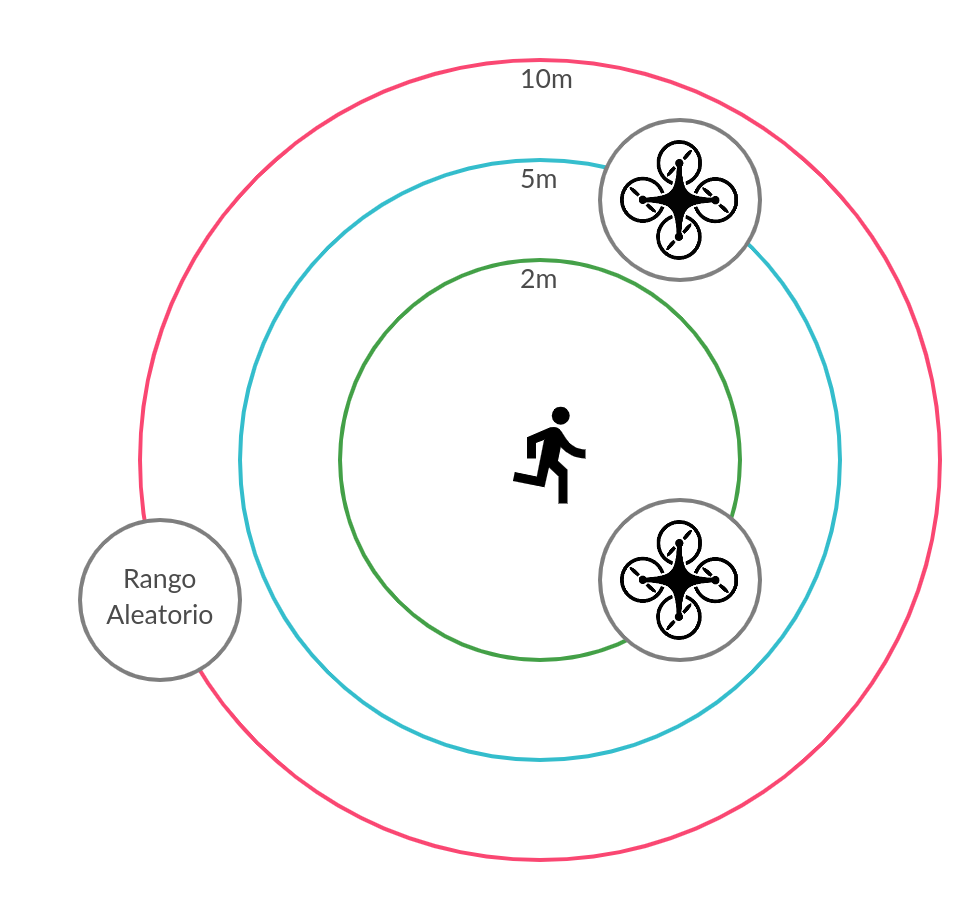
\includegraphics[width=0.6\textwidth]{figures/simulado/capturas.png}
		\caption{función \textit{Esquema de capturas}}
		\label{fig:esquemaCapturas}
		\end{center}
\end{figure}
Una vez generadas todas las capturas se han etiquetado manualmente, primero se han subido a la web \textit{LabelMe} que permite etiquetar las imágenes (figura\ref{fig:datasetlabelme}).
\begin{figure}[H]
  \begin{center}
    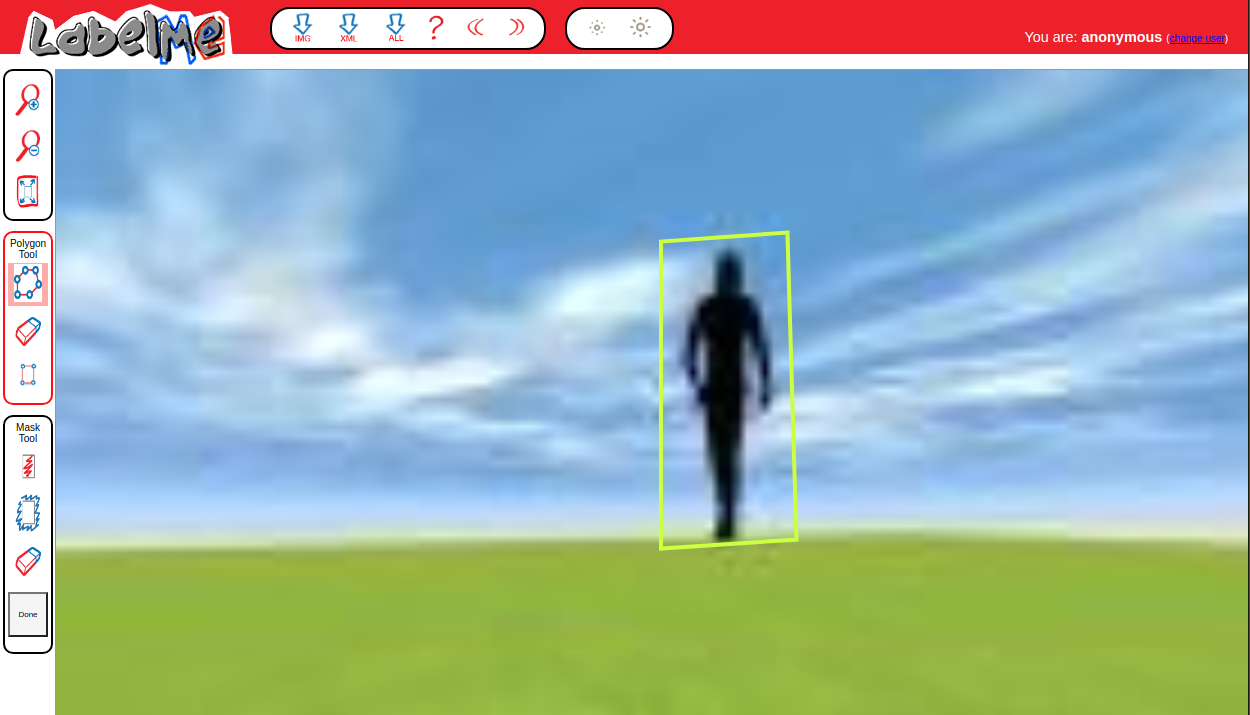
\includegraphics[width=0.6\textwidth]{figures/herramientas/labelme.png}
		\caption{Etiquetado del \textit{dataset} en  \textit{LabelMe}}
		\label{fig:datasetlabelme}
		\end{center}
\end{figure}
Cuando están todas etiquetadas, se descargan, son un conjunto de imágenes y ficheros \textit{XML}.

Para aumentar el tamaño se ha procedido  a espejar las imágenes ya etiquetadas mediante un \textit{script} de \textit{python}, doblando el tamaño de \textit{dataset}. Después de esto se ha dividido en \textit{train} y \textit{test}, dejando un 10\% para la segunda parte mediante otro \textit{script}.

Los dos últimos pasos han sido convertir esos ficheros \textit{XML} en uno \textit{CSV} para \textit{train} y otro para \textit{test} para poder manejar mejor el \textit{dataset} y crear ficheros \textit{record} (ficheros binarios que contienen tanto imágenes como anotaciones) para poderlos usar mejor en los entrenamientos.
\section{Reentrenar red}
El reentrnamiento se ha efectuado en \textbf{google colab} mediante un cuadernillo \textit{python}. La primera intención fue hacerse con \textit{Tensorflow 2.0} pero \textit{Object Detection API} todavía no tiene soporte para guardar las redes entrenadas en formato grafo, por lo que no ha podido usarse en el navegador al tener unos tiempos de detección superiores al segundo.

Para subsanar este contratiempo se ha desarrollado uno equivalente para \textit{Tensorflow 1.15}, donde sí hay soporte. Dicho entrenamiento ha consistido en 20.000 iteraciones con un \textit{batch} de 24 imágenes.
se han obtenido los siguientes resultados: 
\begin{table}[H]
\centering
\begin{tabular}{|c|c|}

\multicolumn{2}{c}{\textbf{Resultados}} \\ \hline
Precision             & 0.64            \\ \hline
Recall                & 0.69            \\ \hline
\end{tabular}
\caption{Resultados del entrenamiento}
\label{tab:cambios_python_2_3}
\end{table}

Además se han obtenido una perdida del 0.3.
Con estos datos junto con una pequeña bajada del limite de confianza se ha conseguido que la detección en el simulador ronde el 80\%. De esta manera ya es posible seguir la persona sin problemas.
\section{Validación experimental}
La validación experimental del desarrollo se ha hecho en 3 casos, uno por cada \textit{PID} y el conjunto. En todos los casos el bucle de control funciona a 7 \acrshort{fps}.

\subsection*{Control de giro horizontal}
Esta prueba consiste en colocar uno de los modelos 3D moviéndose de izquierda a derecha delante del drone, mediante una animación. Permite ajustar las constantes del \textit{PID} de giro horizontal (figuras \ref{fig:SimIzq} y \ref{fig:SimDer}).

\begin{figure}[!htb]
\minipage{0.45\textwidth}
    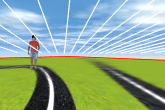
\includegraphics[width=\linewidth]{figures/simulado/izq.png}
    \caption{Modelo a la izquierda}\label{fig:SimIzq}
\endminipage\hfill
\minipage{0.45\textwidth}
    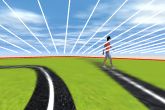
\includegraphics[width=\linewidth]{figures/simulado/der.png}
    \caption{Modelo a la derecha}\label{fig:SimDer}
\endminipage\hfill
\end{figure}

\subsection*{Control de avance}
Esta prueba consiste en colocar uno de los modelos 3D alejándose y acercándose al drone para ajustar las constantes del \textit{PID} de avance (figuras \ref{fig:SimCer} y \ref{fig:SimLej}).

\begin{figure}[!htb]
\minipage{0.45\textwidth}
    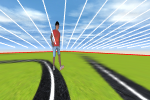
\includegraphics[width=\linewidth]{figures/simulado/cerca.png}
    \caption{Modelo cerca}\label{fig:SimCer}
\endminipage\hfill
\minipage{0.45\textwidth}
    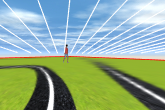
\includegraphics[width=\linewidth]{figures/simulado/lejos.png}
    \caption{Modelo lejos}\label{fig:SimLej}
\endminipage\hfill
\end{figure}
\subsection*{Ejecución típica completa}
En este caso en vez de usar una animación, se le ha conectado un teleoperador existente en \textit{Websim}, que permite controlar un objeto con las flechas del teclado, para poder mover libremente el modelo 3D para que lo siga el \textit{drone} (figura \ref{fig:ejecucion_sim}). si el movimiento no es el esperado, toca ajustar las constantes oportunas.

\begin{figure}[H]
  \begin{center}
    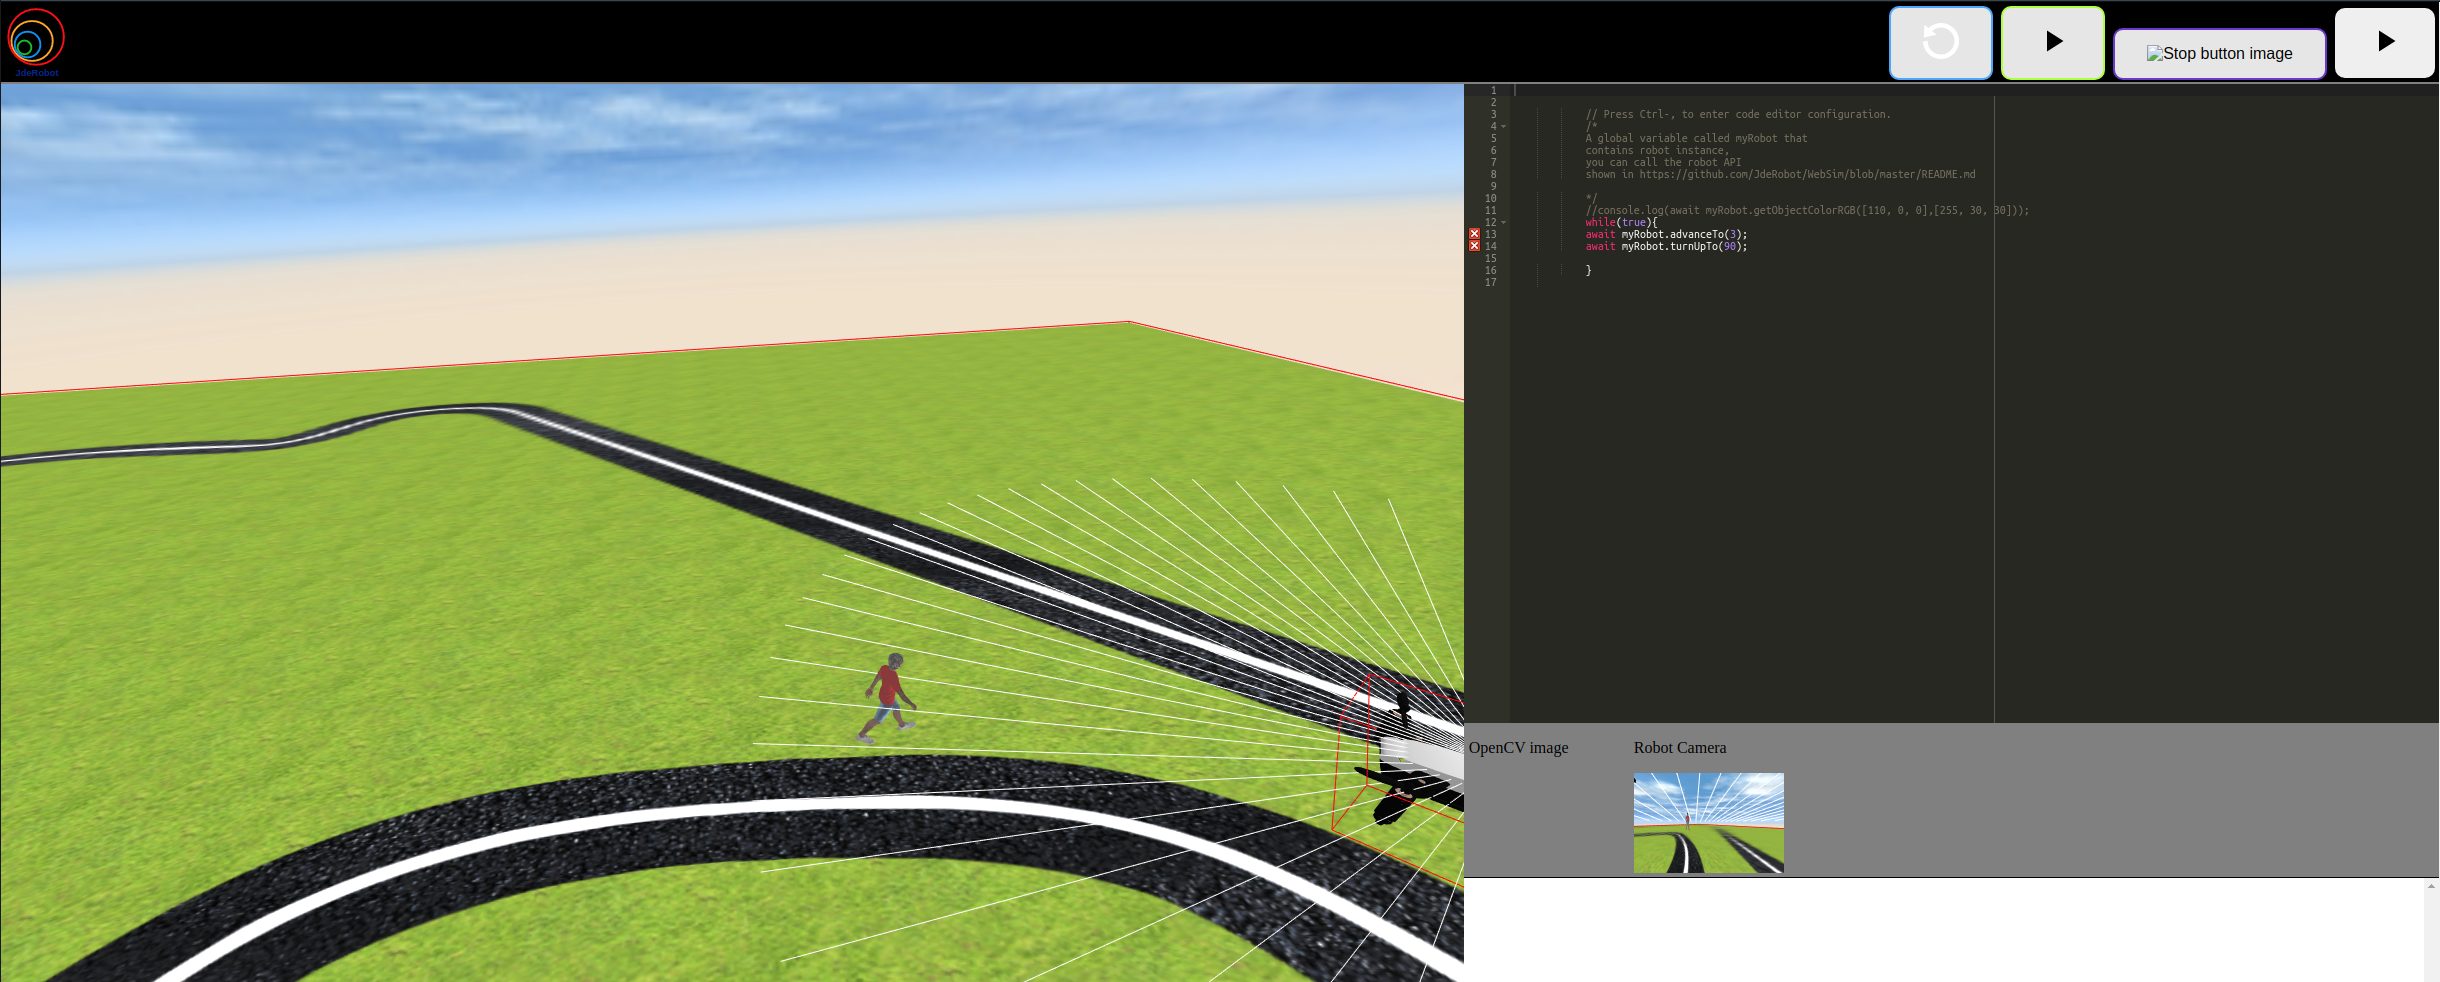
\includegraphics[width=1\textwidth]{figures/simulado/ejemplo1.png}
		\caption{Ejecución Típica}
		\label{fig:ejecucion_sim}
		\end{center}
\end{figure}


